% Generated by opusdb.benchmark.report
% Required packages: \usepackage{pgfplots} \pgfplotsset{compat=1.18}
%                    \usepackage{booktabs} (for throughput tables)

\begin{table}[htbp]
  \centering
  \caption{Throughput: High Contention (single shared ref)}
  \begin{tabular}{@{}rrrr@{}}
    \toprule
    Threads & TPS & Aborts/commit & Correct \\
    \midrule
    4 & 191,989 & 0.00 & \checkmark \\
    6 & 313,780 & 0.00 & \checkmark \\
    12 & 398,005 & 0.07 & \checkmark \\
    \bottomrule
  \end{tabular}
\end{table}

\begin{figure}[htbp]
  \centering
  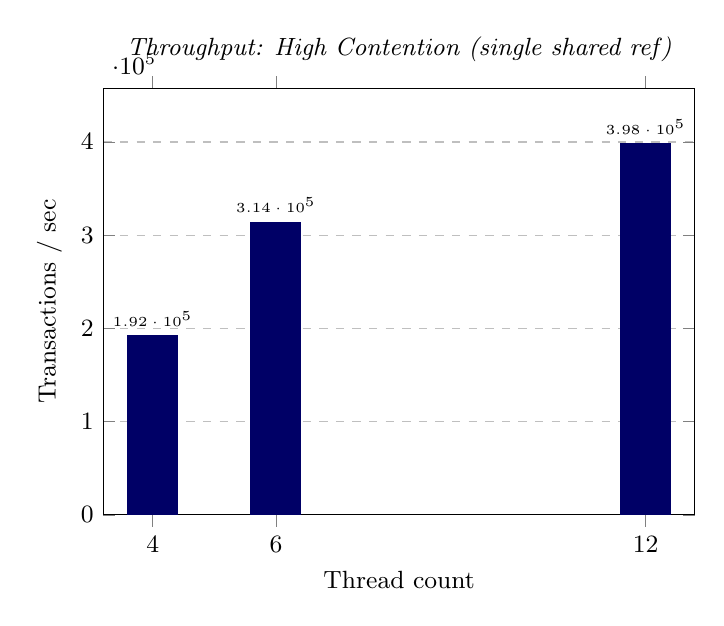
\begin{tikzpicture}
    \begin{axis}[
      title={Throughput: High Contention (single shared ref)},
      xlabel={Thread count}, ylabel={Transactions / sec},
      ybar, bar width=18pt, width=0.75\textwidth, height=7cm,
      xtick=data, ymin=0, enlarge y limits={upper, value=0.15},
      ymajorgrids=true, grid style=dashed,
      nodes near coords, nodes near coords align={vertical},
      every node near coord/.append style={font=\tiny, anchor=south},
      tick label style={font=\small}, label style={font=\small},
      title style={font=\small\itshape}, clip=false,
    ]
    \addplot[fill=blue!40!black, draw=blue!40!black] coordinates {
      (4,191989)
      (6,313780)
      (12,398005)
    };
    \end{axis}
  \end{tikzpicture}
  \caption{Throughput: High Contention (single shared ref)}
  \label{fig:throughput-high-contention}
\end{figure}

\begin{figure}[htbp]
  \centering
  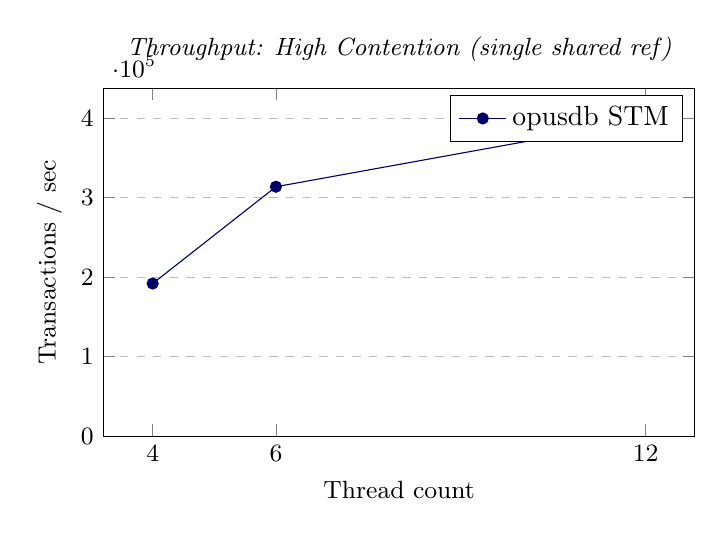
\begin{tikzpicture}
    \begin{axis}[
      title={Throughput: High Contention (single shared ref)},
      xlabel={Thread count},
      ylabel={Transactions / sec},
      width=0.75\textwidth, height=6cm,
      xtick=data, ymin=0,
      ymajorgrids=true, grid style=dashed,
      mark=*, tick label style={font=\small},
      label style={font=\small}, title style={font=\small\itshape},
    ]
    \addplot[color=blue!40!black, mark=*] coordinates {
      (4,191989)
      (6,313780)
      (12,398005)
    };
    \legend{opusdb STM}
    \end{axis}
  \end{tikzpicture}
  \caption{Throughput: High Contention (single shared ref) (Scaling)}
  \label{fig:throughput-high-contention-scaling}
\end{figure}

\begin{figure}[htbp]
  \centering
  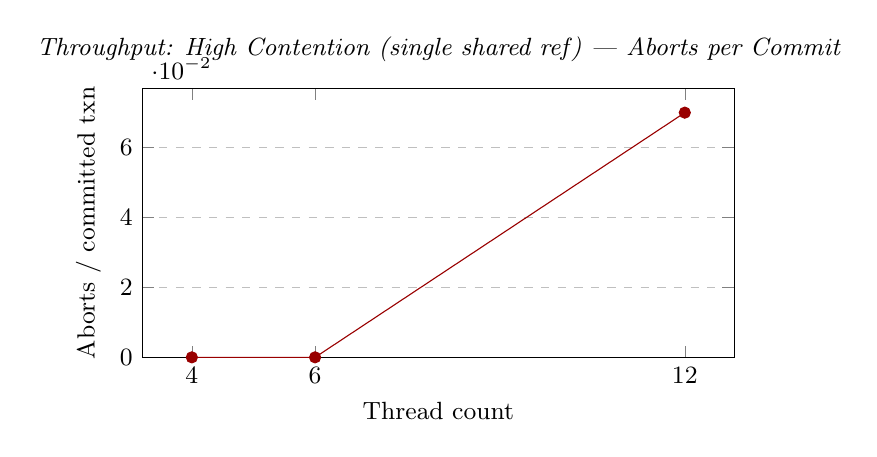
\begin{tikzpicture}
    \begin{axis}[
      title={Throughput: High Contention (single shared ref) — Aborts per Commit},
      xlabel={Thread count},
      ylabel={Aborts / committed txn},
      width=0.75\textwidth, height=5cm,
      xtick=data, ymin=0,
      ymajorgrids=true, grid style=dashed,
      mark=*, tick label style={font=\small},
      label style={font=\small}, title style={font=\small\itshape},
    ]
    \addplot[color=red!60!black, mark=*] coordinates {
      (4,0.00)
      (6,0.00)
      (12,0.07)
    };
    \end{axis}
  \end{tikzpicture}
  \caption{Throughput: High Contention (single shared ref) — Aborts per Commit}
  \label{fig:throughput-high-contention-aborts}
\end{figure}


\begin{table}[htbp]
  \centering
  \caption{Throughput: Low Contention (isolated refs)}
  \begin{tabular}{@{}rrr@{}}
    \toprule
    Threads & TPS & Correct \\
    \midrule
    4 & 1,145,772 & \checkmark \\
    6 & 1,243,557 & \checkmark \\
    12 & 1,360,233 & \checkmark \\
    \bottomrule
  \end{tabular}
\end{table}

\begin{figure}[htbp]
  \centering
  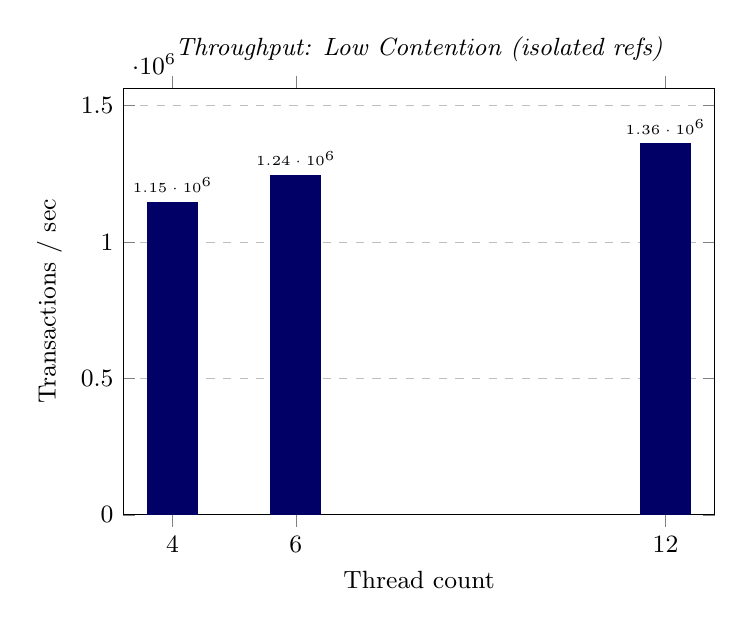
\begin{tikzpicture}
    \begin{axis}[
      title={Throughput: Low Contention (isolated refs)},
      xlabel={Thread count}, ylabel={Transactions / sec},
      ybar, bar width=18pt, width=0.75\textwidth, height=7cm,
      xtick=data, ymin=0, enlarge y limits={upper, value=0.15},
      ymajorgrids=true, grid style=dashed,
      nodes near coords, nodes near coords align={vertical},
      every node near coord/.append style={font=\tiny, anchor=south},
      tick label style={font=\small}, label style={font=\small},
      title style={font=\small\itshape}, clip=false,
    ]
    \addplot[fill=blue!40!black, draw=blue!40!black] coordinates {
      (4,1145772)
      (6,1243557)
      (12,1360233)
    };
    \end{axis}
  \end{tikzpicture}
  \caption{Throughput: Low Contention (isolated refs)}
  \label{fig:throughput-low-contention}
\end{figure}

\begin{figure}[htbp]
  \centering
  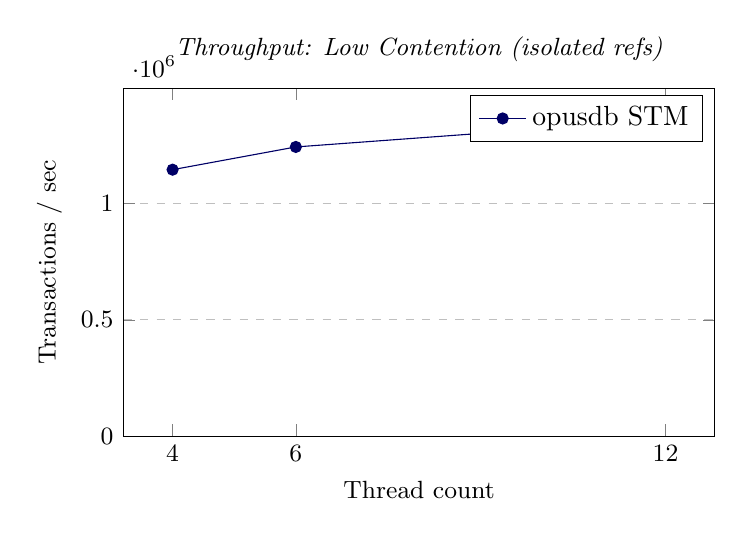
\begin{tikzpicture}
    \begin{axis}[
      title={Throughput: Low Contention (isolated refs)},
      xlabel={Thread count},
      ylabel={Transactions / sec},
      width=0.75\textwidth, height=6cm,
      xtick=data, ymin=0,
      ymajorgrids=true, grid style=dashed,
      mark=*, tick label style={font=\small},
      label style={font=\small}, title style={font=\small\itshape},
    ]
    \addplot[color=blue!40!black, mark=*] coordinates {
      (4,1145772)
      (6,1243557)
      (12,1360233)
    };
    \legend{opusdb STM}
    \end{axis}
  \end{tikzpicture}
  \caption{Throughput: Low Contention (isolated refs) (Scaling)}
  \label{fig:throughput-low-contention-scaling}
\end{figure}


\begin{table}[htbp]
  \centering
  \caption{Throughput: Bank Transfer (20 accounts)}
  \begin{tabular}{@{}rrr@{}}
    \toprule
    Threads & TPS & Correct \\
    \midrule
    4 & 211,423 & \checkmark \\
    6 & 171,684 & \checkmark \\
    12 & 245,861 & \checkmark \\
    \bottomrule
  \end{tabular}
\end{table}

\begin{figure}[htbp]
  \centering
  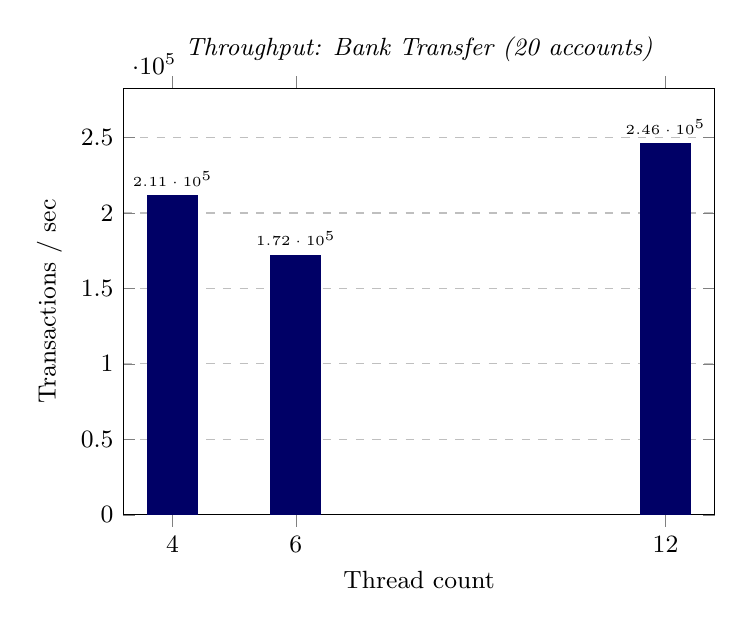
\begin{tikzpicture}
    \begin{axis}[
      title={Throughput: Bank Transfer (20 accounts)},
      xlabel={Thread count}, ylabel={Transactions / sec},
      ybar, bar width=18pt, width=0.75\textwidth, height=7cm,
      xtick=data, ymin=0, enlarge y limits={upper, value=0.15},
      ymajorgrids=true, grid style=dashed,
      nodes near coords, nodes near coords align={vertical},
      every node near coord/.append style={font=\tiny, anchor=south},
      tick label style={font=\small}, label style={font=\small},
      title style={font=\small\itshape}, clip=false,
    ]
    \addplot[fill=blue!40!black, draw=blue!40!black] coordinates {
      (4,211423)
      (6,171684)
      (12,245861)
    };
    \end{axis}
  \end{tikzpicture}
  \caption{Throughput: Bank Transfer (20 accounts)}
  \label{fig:throughput-bank-transfer}
\end{figure}

\begin{figure}[htbp]
  \centering
  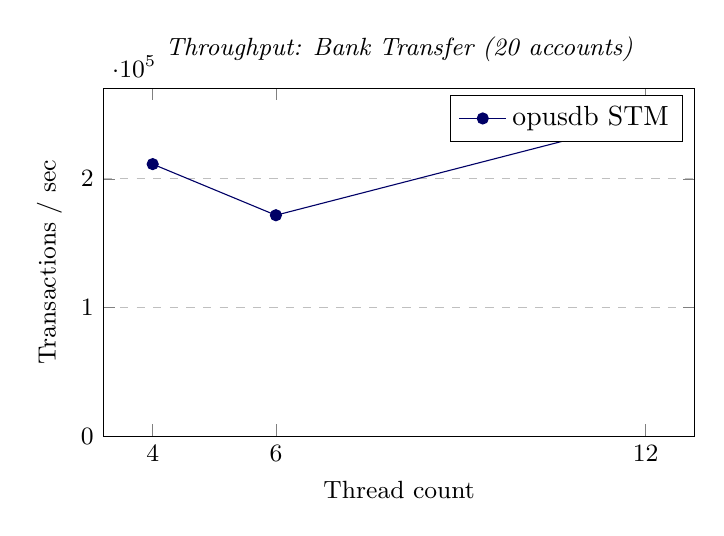
\begin{tikzpicture}
    \begin{axis}[
      title={Throughput: Bank Transfer (20 accounts)},
      xlabel={Thread count},
      ylabel={Transactions / sec},
      width=0.75\textwidth, height=6cm,
      xtick=data, ymin=0,
      ymajorgrids=true, grid style=dashed,
      mark=*, tick label style={font=\small},
      label style={font=\small}, title style={font=\small\itshape},
    ]
    \addplot[color=blue!40!black, mark=*] coordinates {
      (4,211423)
      (6,171684)
      (12,245861)
    };
    \legend{opusdb STM}
    \end{axis}
  \end{tikzpicture}
  \caption{Throughput: Bank Transfer (20 accounts) (Scaling)}
  \label{fig:throughput-bank-transfer-scaling}
\end{figure}


\begin{table}[htbp]
  \centering
  \caption{Throughput: Read-Heavy Mix (10\% writes)}
  \begin{tabular}{@{}rrr@{}}
    \toprule
    Threads & TPS & Correct \\
    \midrule
    4 & 1,454,270 & \checkmark \\
    6 & 1,773,016 & \checkmark \\
    12 & 1,525,335 & \checkmark \\
    \bottomrule
  \end{tabular}
\end{table}

\begin{figure}[htbp]
  \centering
  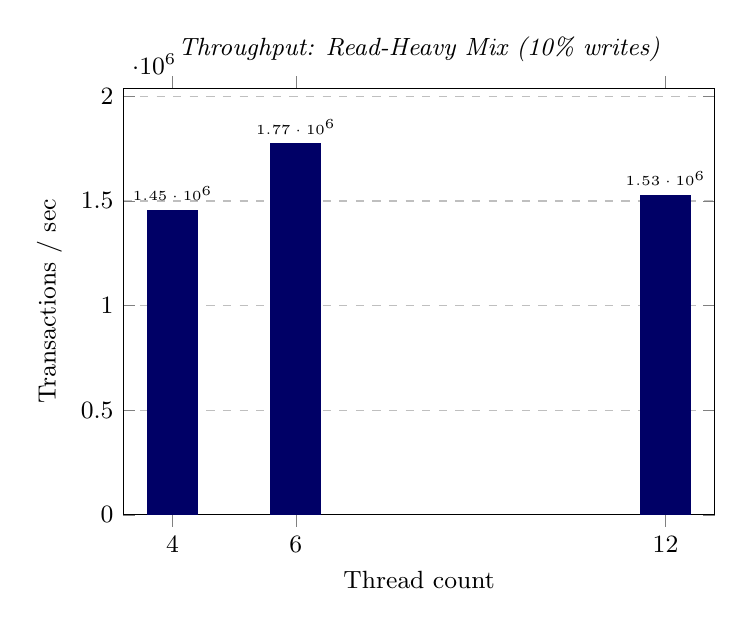
\begin{tikzpicture}
    \begin{axis}[
      title={Throughput: Read-Heavy Mix (10\% writes)},
      xlabel={Thread count}, ylabel={Transactions / sec},
      ybar, bar width=18pt, width=0.75\textwidth, height=7cm,
      xtick=data, ymin=0, enlarge y limits={upper, value=0.15},
      ymajorgrids=true, grid style=dashed,
      nodes near coords, nodes near coords align={vertical},
      every node near coord/.append style={font=\tiny, anchor=south},
      tick label style={font=\small}, label style={font=\small},
      title style={font=\small\itshape}, clip=false,
    ]
    \addplot[fill=blue!40!black, draw=blue!40!black] coordinates {
      (4,1454270)
      (6,1773016)
      (12,1525335)
    };
    \end{axis}
  \end{tikzpicture}
  \caption{Throughput: Read-Heavy Mix (10\% writes)}
  \label{fig:throughput-read-heavy}
\end{figure}

\begin{figure}[htbp]
  \centering
  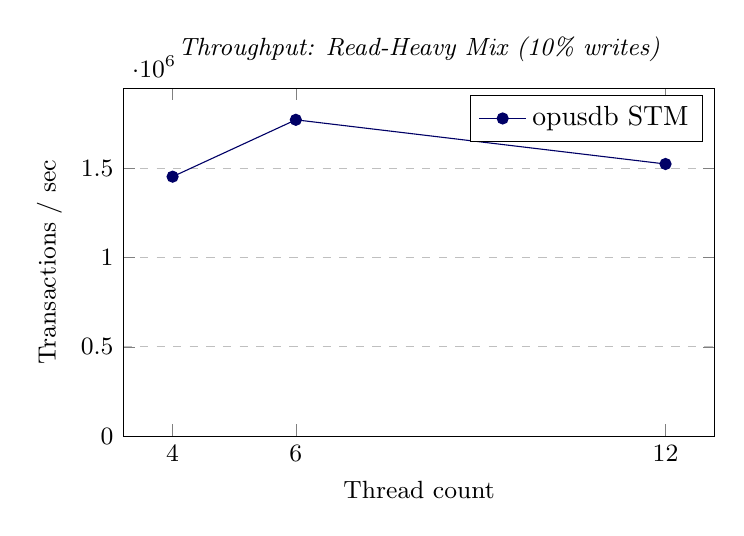
\begin{tikzpicture}
    \begin{axis}[
      title={Throughput: Read-Heavy Mix (10\% writes)},
      xlabel={Thread count},
      ylabel={Transactions / sec},
      width=0.75\textwidth, height=6cm,
      xtick=data, ymin=0,
      ymajorgrids=true, grid style=dashed,
      mark=*, tick label style={font=\small},
      label style={font=\small}, title style={font=\small\itshape},
    ]
    \addplot[color=blue!40!black, mark=*] coordinates {
      (4,1454270)
      (6,1773016)
      (12,1525335)
    };
    \legend{opusdb STM}
    \end{axis}
  \end{tikzpicture}
  \caption{Throughput: Read-Heavy Mix (10\% writes) (Scaling)}
  \label{fig:throughput-read-heavy-scaling}
\end{figure}


\begin{table}[htbp]
  \centering
  \caption{Throughput: Write-Heavy Mix (90\% writes)}
  \begin{tabular}{@{}rrrr@{}}
    \toprule
    Threads & TPS & Aborts/commit & Correct \\
    \midrule
    4 & 587,219 & 0.15 & \checkmark \\
    6 & 617,315 & 0.11 & \checkmark \\
    12 & 543,641 & 0.18 & \checkmark \\
    \bottomrule
  \end{tabular}
\end{table}

\begin{figure}[htbp]
  \centering
  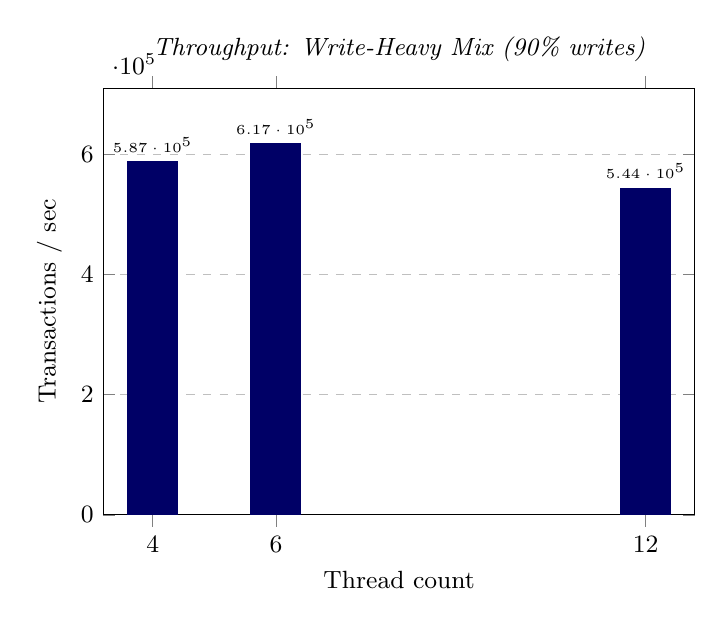
\begin{tikzpicture}
    \begin{axis}[
      title={Throughput: Write-Heavy Mix (90\% writes)},
      xlabel={Thread count}, ylabel={Transactions / sec},
      ybar, bar width=18pt, width=0.75\textwidth, height=7cm,
      xtick=data, ymin=0, enlarge y limits={upper, value=0.15},
      ymajorgrids=true, grid style=dashed,
      nodes near coords, nodes near coords align={vertical},
      every node near coord/.append style={font=\tiny, anchor=south},
      tick label style={font=\small}, label style={font=\small},
      title style={font=\small\itshape}, clip=false,
    ]
    \addplot[fill=blue!40!black, draw=blue!40!black] coordinates {
      (4,587219)
      (6,617315)
      (12,543641)
    };
    \end{axis}
  \end{tikzpicture}
  \caption{Throughput: Write-Heavy Mix (90\% writes)}
  \label{fig:throughput-write-heavy}
\end{figure}

\begin{figure}[htbp]
  \centering
  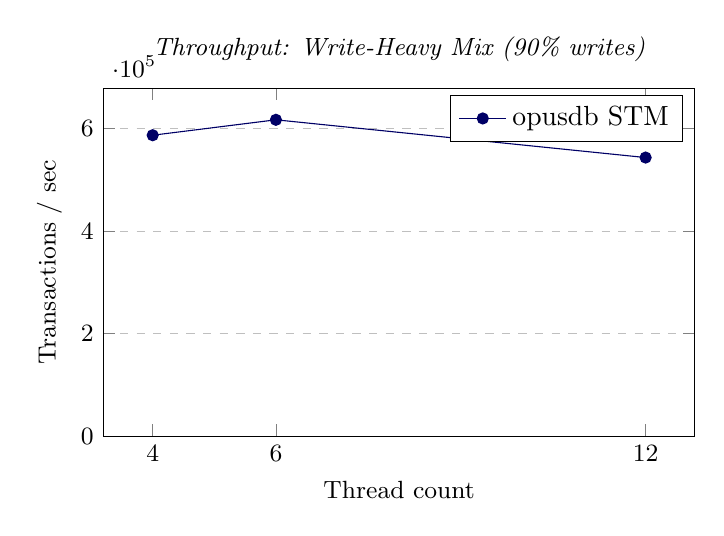
\begin{tikzpicture}
    \begin{axis}[
      title={Throughput: Write-Heavy Mix (90\% writes)},
      xlabel={Thread count},
      ylabel={Transactions / sec},
      width=0.75\textwidth, height=6cm,
      xtick=data, ymin=0,
      ymajorgrids=true, grid style=dashed,
      mark=*, tick label style={font=\small},
      label style={font=\small}, title style={font=\small\itshape},
    ]
    \addplot[color=blue!40!black, mark=*] coordinates {
      (4,587219)
      (6,617315)
      (12,543641)
    };
    \legend{opusdb STM}
    \end{axis}
  \end{tikzpicture}
  \caption{Throughput: Write-Heavy Mix (90\% writes) (Scaling)}
  \label{fig:throughput-write-heavy-scaling}
\end{figure}

\begin{figure}[htbp]
  \centering
  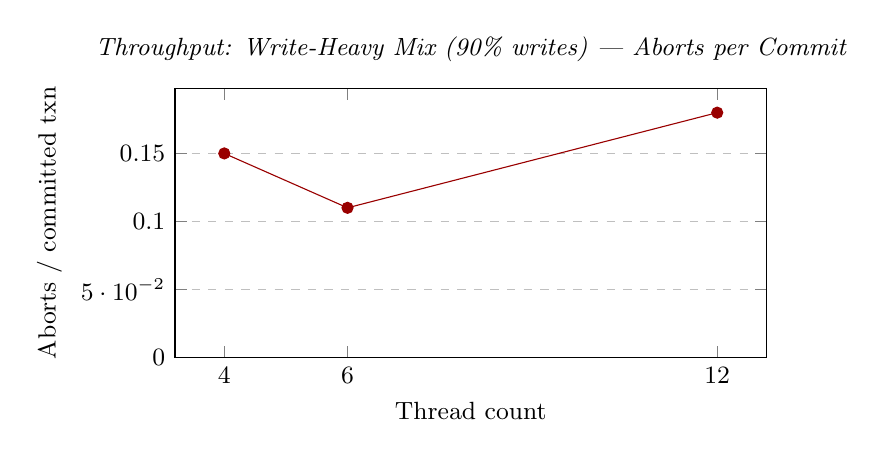
\begin{tikzpicture}
    \begin{axis}[
      title={Throughput: Write-Heavy Mix (90\% writes) — Aborts per Commit},
      xlabel={Thread count},
      ylabel={Aborts / committed txn},
      width=0.75\textwidth, height=5cm,
      xtick=data, ymin=0,
      ymajorgrids=true, grid style=dashed,
      mark=*, tick label style={font=\small},
      label style={font=\small}, title style={font=\small\itshape},
    ]
    \addplot[color=red!60!black, mark=*] coordinates {
      (4,0.15)
      (6,0.11)
      (12,0.18)
    };
    \end{axis}
  \end{tikzpicture}
  \caption{Throughput: Write-Heavy Mix (90\% writes) — Aborts per Commit}
  \label{fig:throughput-write-heavy-aborts}
\end{figure}

\begin{figure}[htbp]
  \centering
  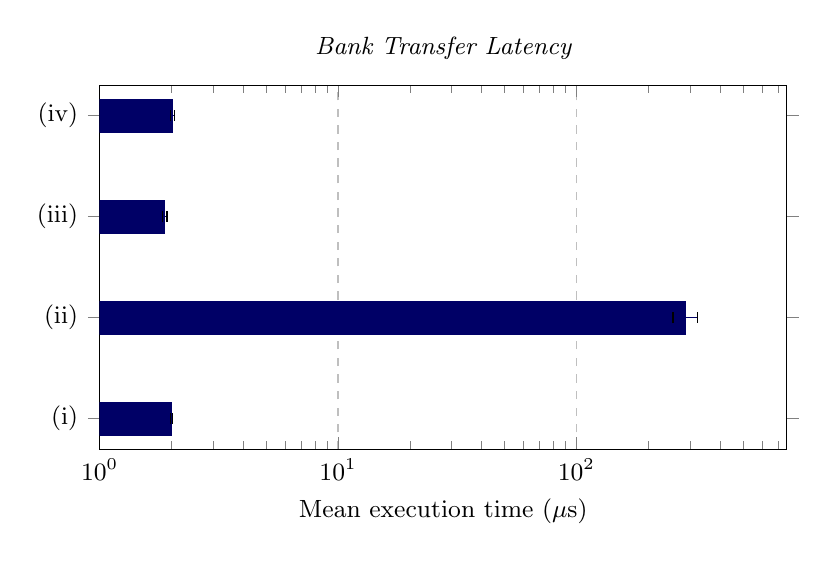
\begin{tikzpicture}
    \begin{axis}[
      title={Bank Transfer Latency},
      xlabel={Mean execution time ($\mu$s)},
      width=0.85\textwidth, height=6.2cm,
      xbar, bar width=12pt, xmode=log, xmin=1,
      enlarge x limits={upper, value=0.15},
      ytick={0,1,2,3},
      yticklabels={(\romannumeral 1),(\romannumeral 2),(\romannumeral 3),(\romannumeral 4)},
      xmajorgrids=true, grid style=dashed,
      tick label style={font=\small}, label style={font=\small},
      title style={font=\small\itshape},
    ]
    \addplot[fill=blue!40!black, draw=blue!40!black,
      error bars/.cd, x dir=both, x explicit
    ] coordinates {
      (1.999,0) +- (0.021,0)
      (287.702,1) +- (33.428,0)
      (1.877,2) +- (0.039,0)
      (2.019,3) +- (0.033,0)
    };
    \end{axis}
  \end{tikzpicture}
  \vspace{0.5em}
  \begin{minipage}{0.85\textwidth}
    \centering \small
    \begin{tabular}{@{}r l@{}}
      (\romannumeral 1) & single transfer transaction — opusdb \\
      (\romannumeral 2) & extreme-contention with futures — opusdb \\
      (\romannumeral 3) & on-commit hook overhead (no hook baseline) — opusdb \\
      (\romannumeral 4) & on-commit hook overhead (with hook) — opusdb \\
    \end{tabular}
  \end{minipage}
  \caption{Bank Transfer Latency}
  \label{fig:bank-contention-latency}
\end{figure}
